\documentclass[11pt]{article}
\usepackage[margin=1in]{geometry}
\usepackage{amsmath,amssymb,amsthm}
\usepackage{graphicx}
\usepackage{array}
\usepackage{xr}
\externaldocument[P-]{tit-rate-leakage}
\usepackage[hidelinks]{hyperref}
\def\UrlBreaks{\do\_\do\.\do\-\do\/}

\newcommand{\R}{\mathbb{R}}
\newcommand{\E}{\mathbb{E}}
\newcommand{\Kc}{\Sigma_{T\mid S}}
\newcommand{\hY}{\hat Y}
\newcommand{\Th}[1]{Theorem~\ref{P-#1}}
\newcommand{\Pp}[1]{Proposition~\ref{P-#1}}
\newcommand{\Co}[1]{Corollary~\ref{P-#1}}
\newcommand{\Se}[1]{Section~\ref{P-#1}}

\title{What One Description Conveys to Each Observer.\\[4pt]
\large An Observation Theory Companion to ``Rate, Leakage, and Distortion for Gaussian Sources''}
\author{Andrew H. Bond\\ San Jos\'e State University}
\date{Draft, October 2026}

\begin{document}
\maketitle

\begin{abstract}
A description of data is usually written for one reader and then held
by others. Observation Theory treats every party that holds a
description as an observer with its own view of the source, its own
geometry for weighing errors, and its own budget, and it asks what the
same description conveys to each of them. This supplement reads the
results of a companion paper on Gaussian sources in that language. The
paper's theorems are stated and proved there in standard information
theory, and nothing here adds to them. All of the results can be
stated with standard source-coding objects. What this supplement adds is
an interpretation. Observation Theory motivated four of the questions,
and it reads their answers as statements about observers. What a
description conveys to an observer is not fixed by what that observer
sees. A tradeoff between the two costs requires the constraints to leave
the encoder a choice among relevant error covariances. In the Gaussian
model, the best one-dimensional description reads a direction that turns
with the budget, which no single-party Gaussian problem with a fixed
weighted quadratic distortion reproduces. And the description that
conveys least to an observer at a given rate is the one that also
describes what that observer sees. The rest of the paper, including its
region and its convexity, is standard and owes nothing to the
interpretation.
\end{abstract}

\section{One description, two observers}
\label{sec:intro}

An encoder sees a source and writes a description for a decoder that
must reconstruct part of it. A second party holds the same description
together with its own noisy view of the source, and it never decodes.
Both parties are observers of one description. The decoder is the
observer the description was written for. The second party is an
observer the description was not written for, and what the description
conveys to it is the information it gains beyond what it already sees.

Standard information theory has the pieces. The rate is what the
decoder pays. What the second party gains is the conditional mutual
information between the source and the description given its view, the
quantity that secure source coding calls the leakage to an eavesdropper.
The region of rates and leakages is known in single-letter form, and
for Gaussian sources the companion paper \cite{paper} works out its
structure.

Observation Theory asks a different question of the same objects. It
asks how the conveyed content depends on who the observer is. The answer
in this setting is that it depends on the observer's geometry as well as
on its data, and the companion paper's theorems make that dependence
exact. This supplement collects four results that Observation Theory
motivated, states what each one says about observers, and marks plainly
which parts of the paper owe nothing to this reading.

\section{The decoder and the second party are both observers}
\label{sec:dictionary}

In Observation Theory an observer is a triple $O=(C,G,B)$. The map $C$
is what the observer reads of the source, the matrix $G$ is the geometry
in which it weighs errors, and $B$ is its budget \cite{obsrep}. The
content a description conveys to an observer that holds side information
is the conditional mutual information between the source and the
description given that side information, the second coordinate of the
rate--content region of \cite{obsrep}.

The companion paper has two observers. The decoder reads $C_1=F$, the
linear part $Y=FT$ of the source it must reconstruct, weighs errors with
$G_1=W$, and has the distortion budget $D$. The second party, called the
holder in the paper, reads $C_2=H$ through the noisy view $S=HT+U$, and
the content conveyed to it is the leakage $I(T;\hY\mid S)$. The encoder
sees the whole source $T$, which may include a context that neither
observer's reconstruction requires. The following table records the
correspondence.

\begin{center}
\begin{tabular}{>{\raggedright\arraybackslash}p{7.2cm}>{\raggedright\arraybackslash}p{7.2cm}}
\hline
Observation Theory & Companion paper \\
\hline
observer the description is written for & decoder, reading $Y=FT$ under weight $W$ \\
observer the description is not written for & holder, seeing $S=HT+U$ \\
content conveyed to an observer with side information & leakage $I(T;\hY\mid S)$ \\
budget of the first observer & distortion budget $D$ \\
geometry of the second observer & information matrix $J=H^{\mathsf T}\Sigma_U^{-1}H$ \\
what the encoder sees & the source $T$, context included \\
\hline
\end{tabular}
\end{center}

Every entry on the right is standard. Secure source coding introduced
the leakage \cite{villard2013}, and the vector Gaussian versions of the
problem were treated by Ekrem and Ulukus \cite{ekrem2013} and by Xu,
Chen, Chen, and Jin \cite{xu2024}. Renaming them does not create a
result, and none of the four findings below depends on this vocabulary.
Each can be stated, and is proved in the companion paper, with standard
source-coding objects. The contribution of Observation Theory here is
that it asked the questions, by treating the second party as an observer
whose geometry matters, and that it gives the answers one coherent
interpretation.

\section{What a description conveys to an observer is not fixed by what the observer sees}
\label{sec:notdetermined}

One might expect the content conveyed to the holder to depend only on
the joint law of what the decoder must reconstruct and what the holder
sees. It does not. The scalar instances in \Se{sec:examples} give two
sources with the same joint law of $(Y,S)$, up to a scaling of $S$, whose
least leakages at the same budget are $1.1880$ and $1.2105$ bits. The
coupled instances give four such sources whose leakage-optimal
descriptions reduce the error along $42.83^\circ$, $37.61^\circ$,
$33.75^\circ$, and $30.84^\circ$ at the same budget.

The difference is the encoder's view. The encoder sees a context that
neither observer reconstructs, and the context is correlated with what
the holder sees. So the content conveyed to the second observer is a
function of three things, the first observer's task, the second
observer's view, and what the writer of the description sees. The joint
law of the two observers' views alone does not determine it. This is the
reason
the companion paper's setting has an encoder that observes more than it
describes.

\section{A tradeoff requires the constraints to leave a choice among error covariances}
\label{sec:scalarbudget}

Suppose the decoder's requirement is a full error covariance on the whole
source, so that every direction must be reconstructed to a prescribed
accuracy. The content conveyed to the holder is still a cost, and it
still depends on the holder. But \Pp{prop:matrix} shows that one
description minimizes the rate and that cost together, so the two costs
do not conflict. The result is implied by the bounds of Ekrem and Ulukus
\cite{ekrem2013}.

The two costs conflict when the constraints leave the encoder a choice
among error covariances that matter to the holder. A weighted total
distortion leaves such a choice, because the encoder decides how to
spread the error over directions. So does a matrix constraint on the
described part alone, which leaves the error free outside that part, as
the companion paper notes after \Pp{prop:matrix}. In the language of
Observation Theory, the first observer's constraints must leave freedom
that the second observer's geometry can act on. Every other result below
lives in that freedom.

\section{The observer's geometry changes what an optimal description reads}
\label{sec:geometry}

This is the central finding. Its scope is the Gaussian model and the
best one-dimensional description, which is the leakage-optimal
description wherever the certificate of the companion paper holds.

A description written for a single observer under a weighted quadratic
distortion reads fixed directions of the source at every budget. The
budget sets how many directions are described and how finely, never
which ones (\Pp{prop:single}). Principal components, reverse
water-filling, and the Gaussian information bottleneck all behave this
way.

When a second observer is present, the best one-dimensional description
reads a direction that turns as the budget changes, unless that
direction is shared by the decoder's geometry and the holder's
(\Th{thm:turning}, which assumes the largest eigenvalue of its pencil is
simple). In the coupled instance the leakage-optimal description reduces
the error along $47.48^\circ$ at one budget and $41.15^\circ$ at another.
\Co{cor:nonred} states what this excludes. No single-party Gaussian
rate--distortion problem with a fixed weighted quadratic distortion has
the leakage-optimal descriptions as its optimal descriptions at two such
budgets. It does not exclude every richer single-observer model, such as
one whose distortion measure changes with the budget. Within the stated
class, the turning is the trace of the second observer.

The cost of ignoring it is explicit. A description that keeps a fixed
direction pays an excess in content conveyed to the holder that
\Pp{prop:fixedread} and \Th{thm:forced} bound from below. For a scalar
source with a nearly clean context, every fixed direction conveys at
least $0.0245$ bits more than necessary at one of two budgets, which
exceeds the least leakage $0.0216$ bits at the second budget.

The turning comes from the misalignment of the two observers'
geometries, not from the context. A described variable with no context
at all turns whenever the decoder's weight and the holder's information
share no eigenvector.

\section{To convey little to an observer, describe what that observer sees}
\label{sec:augmented}

The general solution has a reading that is natural in Observation
Theory. \Th{thm:tilted} shows that every frontier description is reverse
water-filling on the decoder's weight tilted by the information the
holder's view adds. \Co{cor:augmented} restates this. The description that conveys least to
the holder at a given rate is the rate--distortion optimal description
for a decoder that must reconstruct the holder's own view as well as its
target, with a weight that the solution itself fixes.

The reason is an identity. The content conveyed to the holder is the
rate minus the information the description carries about what the
holder sees. So a description that already tells the holder much of what
it sees has little left to convey beyond it. In the language of the
theory, the first observer's effective geometry is its own geometry plus
a copy of the second observer's view, weighted by how uncertain that view
remains after the description.

For a scalar described variable this becomes a single explicit curve
(\Th{thm:scalarpath}). Every optimal description, at every budget and
every weighting of the two costs, reads a direction on the path from the
decoder's own target toward the target corrected by the holder's
information. The rate-optimal description sits at one end, and the
description that conveys least sits at a point that moves with the
budget.

\section{On eleven datasets the single-party flip holds, and the two-observer flip holds where the Gaussian model does}
\label{sec:data}

The companion notebook \texttt{ot\_figures/ot\_figures.ipynb} tests two
flips on eleven public datasets, including the Topology Zoo table of a
routing study. For each dataset the roles were fixed before any outcome
was computed and pushed to the public repository on 2 October 2026, and
the run started a minute after the push, as the notebook records. Predictions use the
second-order statistics of a training half. Outcomes use real 3-bit
quantizers on a held-out half. On real data the conditional leakage
$H(M\mid S)$ of a code $M$ cannot be computed, and every measured leakage
in this section is a proxy for it, the cross-entropy of the best of three
classifiers $q(m\mid s)$ that predict the code from the second party's
view. Its population value is
\[
\E[-\log_2 q(M\mid S)]=H(M\mid S)+\E_S\,D\bigl(p(M\mid S)\,\big\|\,q(M\mid S)\bigr),
\]
so it adds the classifier's error to the leakage, and the difference of
two proxies mixes a difference of conditional entropies with a
difference of classifier errors. In these runs the classifier was also
chosen on the same held-out samples on which its loss was reported. The
ordering of two proxies therefore does not establish the ordering of the
true conditional entropies, and the claims below are claims about the
proxy.

The single-party flip holds in all eleven datasets. At matched bits, the
code that reconstructs the whole source worse serves the decoder better.
Its boundary holds as predicted. Both halves of the flip vanish as the
angle between the decoder's task and the source's energy direction goes
to zero, and grow with it (Fig.~\ref{fig:flipA}), although the
whole-source half is noisy below 30 degrees.

The two-observer flip holds at all three budgets in eight datasets and
at two of three in a ninth. At matched bits, the code that reconstructs
the decoder's target worse has the lower leakage proxy at the second
party. It fails in two datasets, a wine-quality table with a discrete
target and the 175-row Topology Zoo table, where the leakage-aware code
had the higher proxy.
Across 115 choices of what the second party sees, the predicted
correlation ranks the leakage removed with a Spearman correlation of
0.62, with a residual at zero correlation. Two further predictions were
refuted and are recorded in the notebook. A view uncorrelated with the
decoder's principal read still yields a flip once the budget has slack,
and a local onset test held in only four of eleven datasets. Both used
the squared correlation with the decoder's principal read as the
predictor. The boundary theory below replaces it with the position of
that read in a pencil of the view, under which an uncorrelated view can
still flip once the budget has slack.

The boundary of the two-observer flip was then registered in two
stages. The theory places it at the position of the decoder's principal
read in a pencil of the second party's view. If that read is the view's
most predictable direction there is no flip at any slack. Otherwise the
flip appears, with a size the Gaussian model predicts. Predictions for
561 cases were pushed with the scoring script before any held-out code
was measured. They cover thirteen sources (the eleven datasets and two
synthetic Gaussian ones), each context column as the second party's
view, a noisy copy of the principal read as a control, and a family of
views rotated away from that read. Two of the four registered criteria
passed. Where the predicted removal is at least 0.10 bit, the measured
removal is positive in 81 percent of 413 cases, and the Spearman
correlation over all cases is 0.67. On the synthetic Gaussian sources
every case agrees with its prediction within two standard errors, and
the control measures zero. Two criteria were not met. Where the
predicted removal is below 0.05 bit, 56 percent of 57 cases fall within
two standard errors of zero, against a registered 80 percent. Within the
rotated family the rank correlation is 0.56, against a registered 0.6.
Nine of the eleven datasets track the prediction with rank correlations
between 0.81 and 0.98. The bike-rental table, whose targets are counts,
ranks its cases correctly at a tenth of the predicted size. The wine and
Topology Zoo tables are again reversed. We read these misses as returns
from the edge of the Gaussian model, and a second registration tests
that reading by asking whether a measured departure from Gaussianity
predicts where they fall.

The leakage predictions rest on one modelling step. What the second
party learns from a code depends on its view only through a linear
correlation, which is exact when the projection and the view are jointly
Gaussian. The second registration measures, on training halves only,
how far each code departs from that step. It adds the information the
view carries beyond the linear correlation to the divergence of the
code's cell occupancies from their Gaussian design, each in bits above
the 95th percentile of a Gaussian null of the same size. On the measured
datasets this index ranks the size of each miss with a Spearman
correlation of 0.71 over 477 cases. It was then applied blind to six
public datasets this program had never touched, with a cut calibrated on
the eleven measured ones. Before any of their codes were measured, it
forecast that a power-plant table, an airfoil-noise table, and a
real-estate table would track the theory, and that a yacht-hydrodynamics
table, a forest-fire table, and a red-wine table would not. All six
forecasts were right. On the fresh cases the index ranks the misses with
a correlation of 0.67, and the cases it cannot tell from Gaussian agree
with their predictions in 16 of 16, against 33 percent of the rest. Two
criteria were not met. A calibration bar asked that 90 percent of the
synthetic Gaussian cases score zero, and 84 percent did. Each case faces
four tests at the 95th percentile, so the bar should have been near 81
percent. A second comparison was vacuous, because no case from the
measured datasets scored zero. The theory's own modelling assumption
thus forecasts where the theory holds. Read after the fact and not as a
test, the two criteria the boundary test missed behave the same way.
Below the cut the rank correlation in the rotated family is 0.77 on the
measured datasets and 0.74 on the fresh ones. Above it the correlation is
0.31 and $-0.15$. The near-boundary criterion is still unmet below the cut on the
measured datasets, at 64 percent.

A third registration tested these readings blind on six more public
datasets, with the departure cut frozen in advance. The forecast was
again right for all six. Inside the Gaussian scope the measured removal
was positive in all 180 cases predicted at 0.10 bit or more, the rank
correlation was 0.97, and the rotated family reached 0.92, so the
criterion the boundary test missed holds inside the scope on new data.
The onset criteria passed, the second-order family staying at zero at
the smallest slack in 4 of 4 cases and the first-order family rising
above it in 4 of 5. The near-boundary criterion failed for the third
time, at 35 percent of 23 cases, so it fails inside the scope as well as
outside it. The registration also tested the deduced account of the
misses. The error of a leakage prediction, measured against the true
conditional entropy, splits exactly into a marginal defect, the mismatch
between a code's cell occupancy and its Gaussian design, and a
dependence defect, the information the view carries beyond its linear
correlation. The proxy adds the classifier's error to both. On the 20 earlier sources the
marginal defect accounted for most of the error. On the new data,
correcting for it did not lower the mean miss, which was 0.096 bit
against 0.092 without the correction. Codes with equal cell occupancy
restored the ranking on the one dataset outside the scope, from $-0.34$
to $0.82$, but agreed with their predictions less often than the
standard codes outside the scope, in 9 percent of cases against 23. A
symbolic-regression search over the earlier sources had found the
squared difference of the two codes' dependence defects as the predictor
of the remaining misses. It did not hold across datasets there and was
only reported, but on the new data it classified 86 percent of cases
correctly, against 63 percent for always predicting no miss. Outside the Gaussian scope the dependence
defect, or the classifier error that the proxy adds, is therefore the
larger unexplained term, and the marginal account of the misses holds
only in part.

A fourth registration asked why the near-boundary criterion keeps
failing. One account held that its standard error, a bootstrap over the
held-out points of a single split, understates the variability of the
measurement. The other held that the measured removal is systematically
nonzero near the boundary. The 71 in-scope near-boundary cases on real
data were measured again on 20 fresh splits. The spread across splits
was smaller than the bootstrap error, at a median ratio of 0.76, so the
first account fails. In half the cases the mean over the splits sat more
than three standard errors from zero, so by the reading fixed in advance
the misses are systematic. A comparison made after the scoring shows
what the criterion had been testing. Its cases are not predicted at
zero. Their predicted removals lie between 0.03 and 0.05 bit, and the
criterion compared the measurement with zero rather than with the
prediction. On synthetic Gaussian sources the mean over splits lies
within 0.006 bit of the prediction, and every single measurement is
within two standard errors of it. On real data inside the scope the
predicted removals of about 0.04 bit do not appear. The mean over splits
sits near zero, and in 80 percent of cases it lies more than three
standard errors from the prediction. So on Gaussian data the proxy
matches the prediction near the boundary, and on real data inside the
scope it falls systematically short of it. These runs do not separate a
misspecified Gaussian model from unequal classifier errors on the two
codes, and the cause of the shortfall is open. A fifth registration tests the corrected
criterion against the prediction, and whether the shortfall on real data
is a fixed offset or a proportional attenuation.

\begin{figure}[t]
\centering
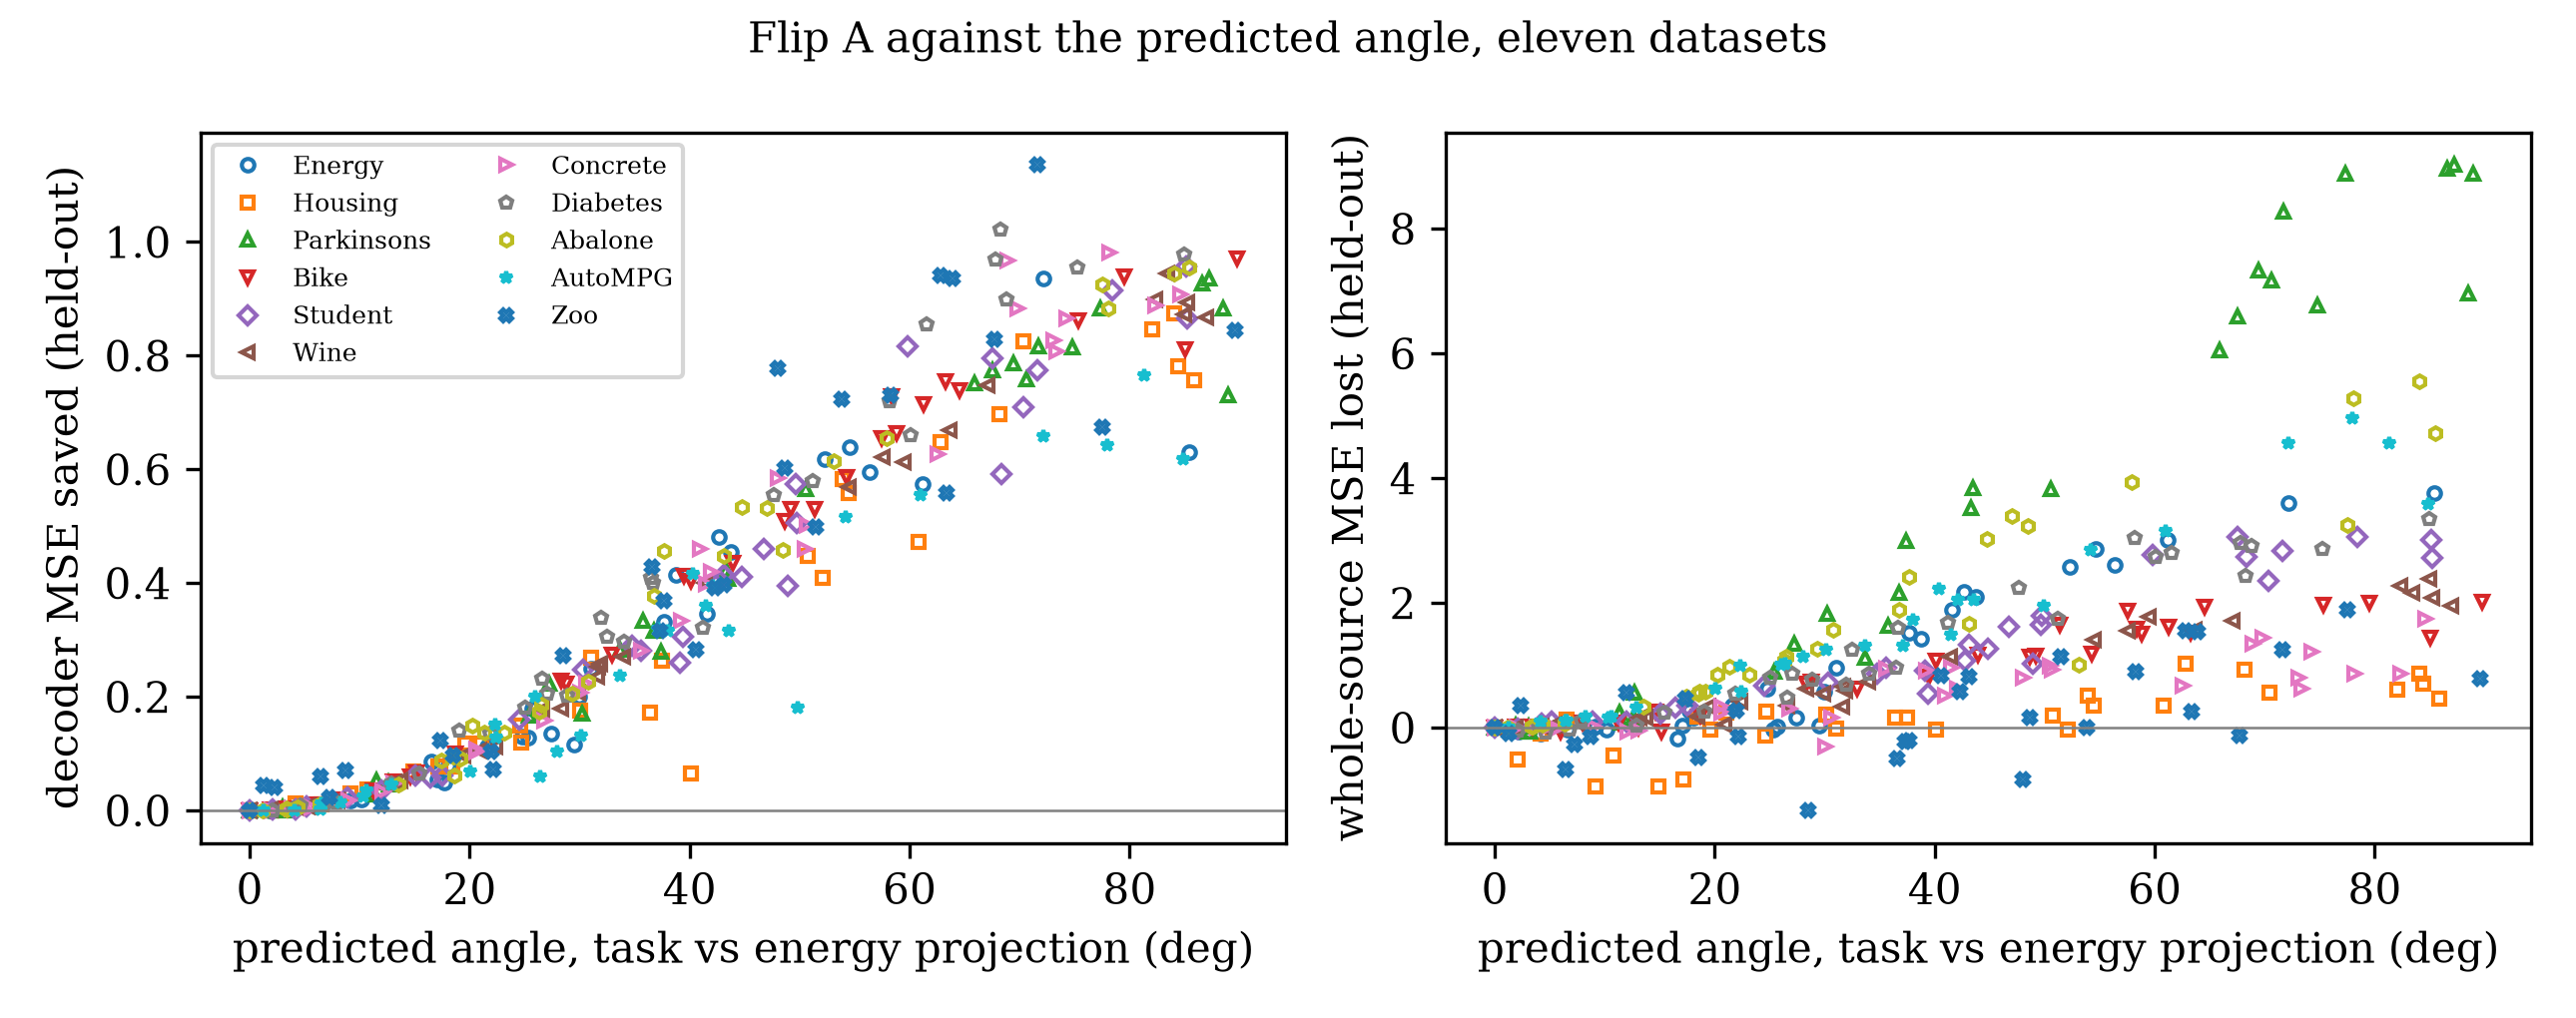
\includegraphics[width=\linewidth]{ot_figures/fig5_flipA_boundary.png}
\caption{The single-party flip on eleven datasets. Each point is one
decoder task. The decoder's gain (left) and the whole-source loss
(right) of the consumer code are both near zero where the training half
predicts alignment, and grow with the predicted angle.}
\label{fig:flipA}
\end{figure}

\paragraph{Experiment ledger.} The companion notebook covers the first
campaign only. Table~\ref{tab:ledger} lists every registration with the
commit at which its code and predictions were frozen and the commit of
its scored outcome, all in the public repository under
\texttt{paper/tit-rate-leakage}.

\begin{table}[t]
\centering
\footnotesize
\caption{Registrations of the empirical campaign. Verdicts are as scored
by the frozen scripts. Every leakage is the classifier cross-entropy
proxy described in Section~\ref{sec:data}.}
\label{tab:ledger}
\begin{tabular}{>{\raggedright\arraybackslash}p{2.4cm}>{\raggedright\arraybackslash}p{4.1cm}>{\raggedright\arraybackslash}p{3.3cm}>{\raggedright\arraybackslash}p{4.6cm}}
\hline
Registration & Frozen code and predictions & Scoring and outcome & Verdicts\\
\hline
Flips A and B & \path{ot_figures.ipynb}, roles on branch \path{prespec/ot-notebook-2026-10-01} & notebook record, \path{9ffbd20} & Flip A 11 of 11, Flip B 8 of 11, onset refuted\\
Boundary of Flip B & \path{ot_boundary.py}, \path{boundary_predictions.json}, \path{7332b8c} & \path{boundary_score.py} (\path{86eccd7}), \path{daca788} & C1 pass, C2 fail, C3 pass, C5 fail\\
Gaussian departure & \path{ot_gaussianity.py} (\path{1441065}), \path{gauss_predictions.json} (\path{ec3300d}) & \path{gauss_score.py}, \path{9f2a61b} & R1 pass, R2 vacuous, K1 fail, B1 pass, B2 pass, B3 6 of 6\\
Gaussian scope & \path{ot_scope.py} (\path{74c446d}), \path{scope_predictions.json} (\path{9f5f2ca}), correction note \path{15cca7b} & \path{scope_score.py}, \path{c14e579} & S0 6 of 6, S1 pass, S2 fail, S3 pass, S4a pass, S4b pass, K1 pass, M1 fail, E1 fail, E2 fail, E3 pass\\
Near-boundary noise & \path{ot_s2noise.py} (\path{fec42f0}) & built into the script, \path{9fa0d23} & N1 fail, N2 fail, B1 pass\\
Corrected near-boundary test & \path{ot_nearboundary.py} (\path{ae487c4}), \path{nb_predictions.json} (\path{3f9d1aa}) & built into the script & pending\\
\hline
\end{tabular}
\end{table}

The deduction of the two defects (\texttt{DEDUCTION-gaussian-defect-2026-10-02.md},
\texttt{c9fcc18}) was committed before it was computed. The mining and
symbolic-regression runs that followed it (\texttt{ot\_mining.py},
\texttt{ot\_radar\_induction.py}) are exploratory and are not
registrations.

\section{What does not need Observation Theory}
\label{sec:standard}

Most of the companion paper is standard information theory, and its
value there does not depend on the reading above. The single-letter
region is due to Villard and Piantanida \cite{villard2013}. Without
decoder side information it is a union of the matrix-distortion regions
of Ekrem and Ulukus \cite{ekrem2013}, and the paper proves the Gaussian
coding theorem directly (\Th{thm:op}). The convexity of both costs in
the error covariance (\Th{thm:convex}), the dimension bound
(\Pp{prop:rank}), the closed forms in commuting geometry and at low
distortion (\Th{thm:commuting}, \Th{thm:lowdist}), the one-dimensional
pencil (\Th{thm:onedim}), and the monotone iteration (\Pp{prop:mm}) are results about
a convex program. They would be stated the same way by a reader who had
never heard of observers.

\section{Open questions about several observers}
\label{sec:open}

The companion paper has one observer the description is written for and
one it is not. Observation Theory asks the same questions of more.

\emph{Several holders.} With holders that see different views, the
content conveyed to each is a separate cost, and the frontier becomes a
surface. A weighted Gaussian objective already gives a sum of tilts, one
per holder, by the argument of \Th{thm:tilted}. The open questions are
operational and geometric. Whether every point of that surface is
achievable needs a coding theorem for several holders at once, and
whether it has explicit solutions, for instance a direction that turns
toward one holder and away from another, is not known.

\emph{Observers on both sides.} When the decoder also has side
information and neither side dominates, the second auxiliary of the
secure source coding region can matter. Xu, Chen, Chen, and Jin
\cite{xu2024} characterize the region under a matrix distortion on the
whole source, stated in the preprint for full-rank views of both
receivers. Whether the observer effects of
Sections~\ref{sec:geometry} and~\ref{sec:augmented} survive under
constraints that leave a choice of error covariance, such as a weighted
total distortion, and a rank-deficient holder is the main open question.

\emph{Observers with rich views.} For a holder whose view has rank above
one and a described variable of dimension above one, the frontier is the
limit of an iteration of closed-form steps (\Pp{prop:mm}) but has no
known closed form.

\emph{Beyond Gaussian sources.} The non-determination of
Section~\ref{sec:notdetermined} and the turning of
Section~\ref{sec:geometry} were found in the Gaussian case. Whether they
hold for finite alphabets, where the single-letter region is also known
\cite{villard2013}, is open.

\section*{Where this fits}

The observer triple and the rate--content region are defined in
\cite{obsrep}, which also treats two observers on one description. The
vector form of the two-observer results, with several described
coordinates, is in \cite{vector}. The scripts that check every number
quoted here are listed in the companion paper's appendix on numerical
checks.

\begin{thebibliography}{9}
\bibitem{paper} A. H. Bond, ``Rate, leakage, and distortion for Gaussian
sources: Water-filling on a tilted weight,'' manuscript, 2026.
\bibitem{obsrep} A. H. Bond, ``Observer representation,'' draft, 2026,
\texttt{paper/observer-representation.tex} in
\texttt{https://github.com/ahb-sjsu/geometric-observation}.
\bibitem{vector} A. H. Bond, ``Rate and conditional content for Gaussian
vector sources with encoder-observed context,'' draft, 2026,
\texttt{paper/tit-vector-described} in the same repository.
\bibitem{villard2013} J. Villard and P. Piantanida, ``Secure multiterminal
source coding with side information at the eavesdropper,'' \emph{IEEE
Trans. Inf. Theory}, vol. 59, no. 6, pp. 3668--3692, 2013.
\bibitem{ekrem2013} E. Ekrem and S. Ulukus, ``Secure lossy transmission of
vector Gaussian sources,'' \emph{IEEE Trans. Inf. Theory}, vol. 59,
no. 9, pp. 5466--5487, 2013.
\bibitem{xu2024} Y. Xu, G. Chen, J. Chen, and S. Jin, ``New proofs of
Gaussian extremal inequalities with applications,'' \emph{IEEE Trans.
Inf. Theory}, vol. 70, no. 5, pp. 3082--3099, 2024.
\end{thebibliography}

\end{document}
